\subsection{Package \lstinline!cryptocast.crypto!}
This package provides basic primitives for working with broadcast encryption protocols
 and useful utilities for working with polynomials over fields, which is necessary to implement
 the Naor-Pinkas scheme.

\noindent\begin{minipage}[t]{5cm}
\vspace{0.3em}
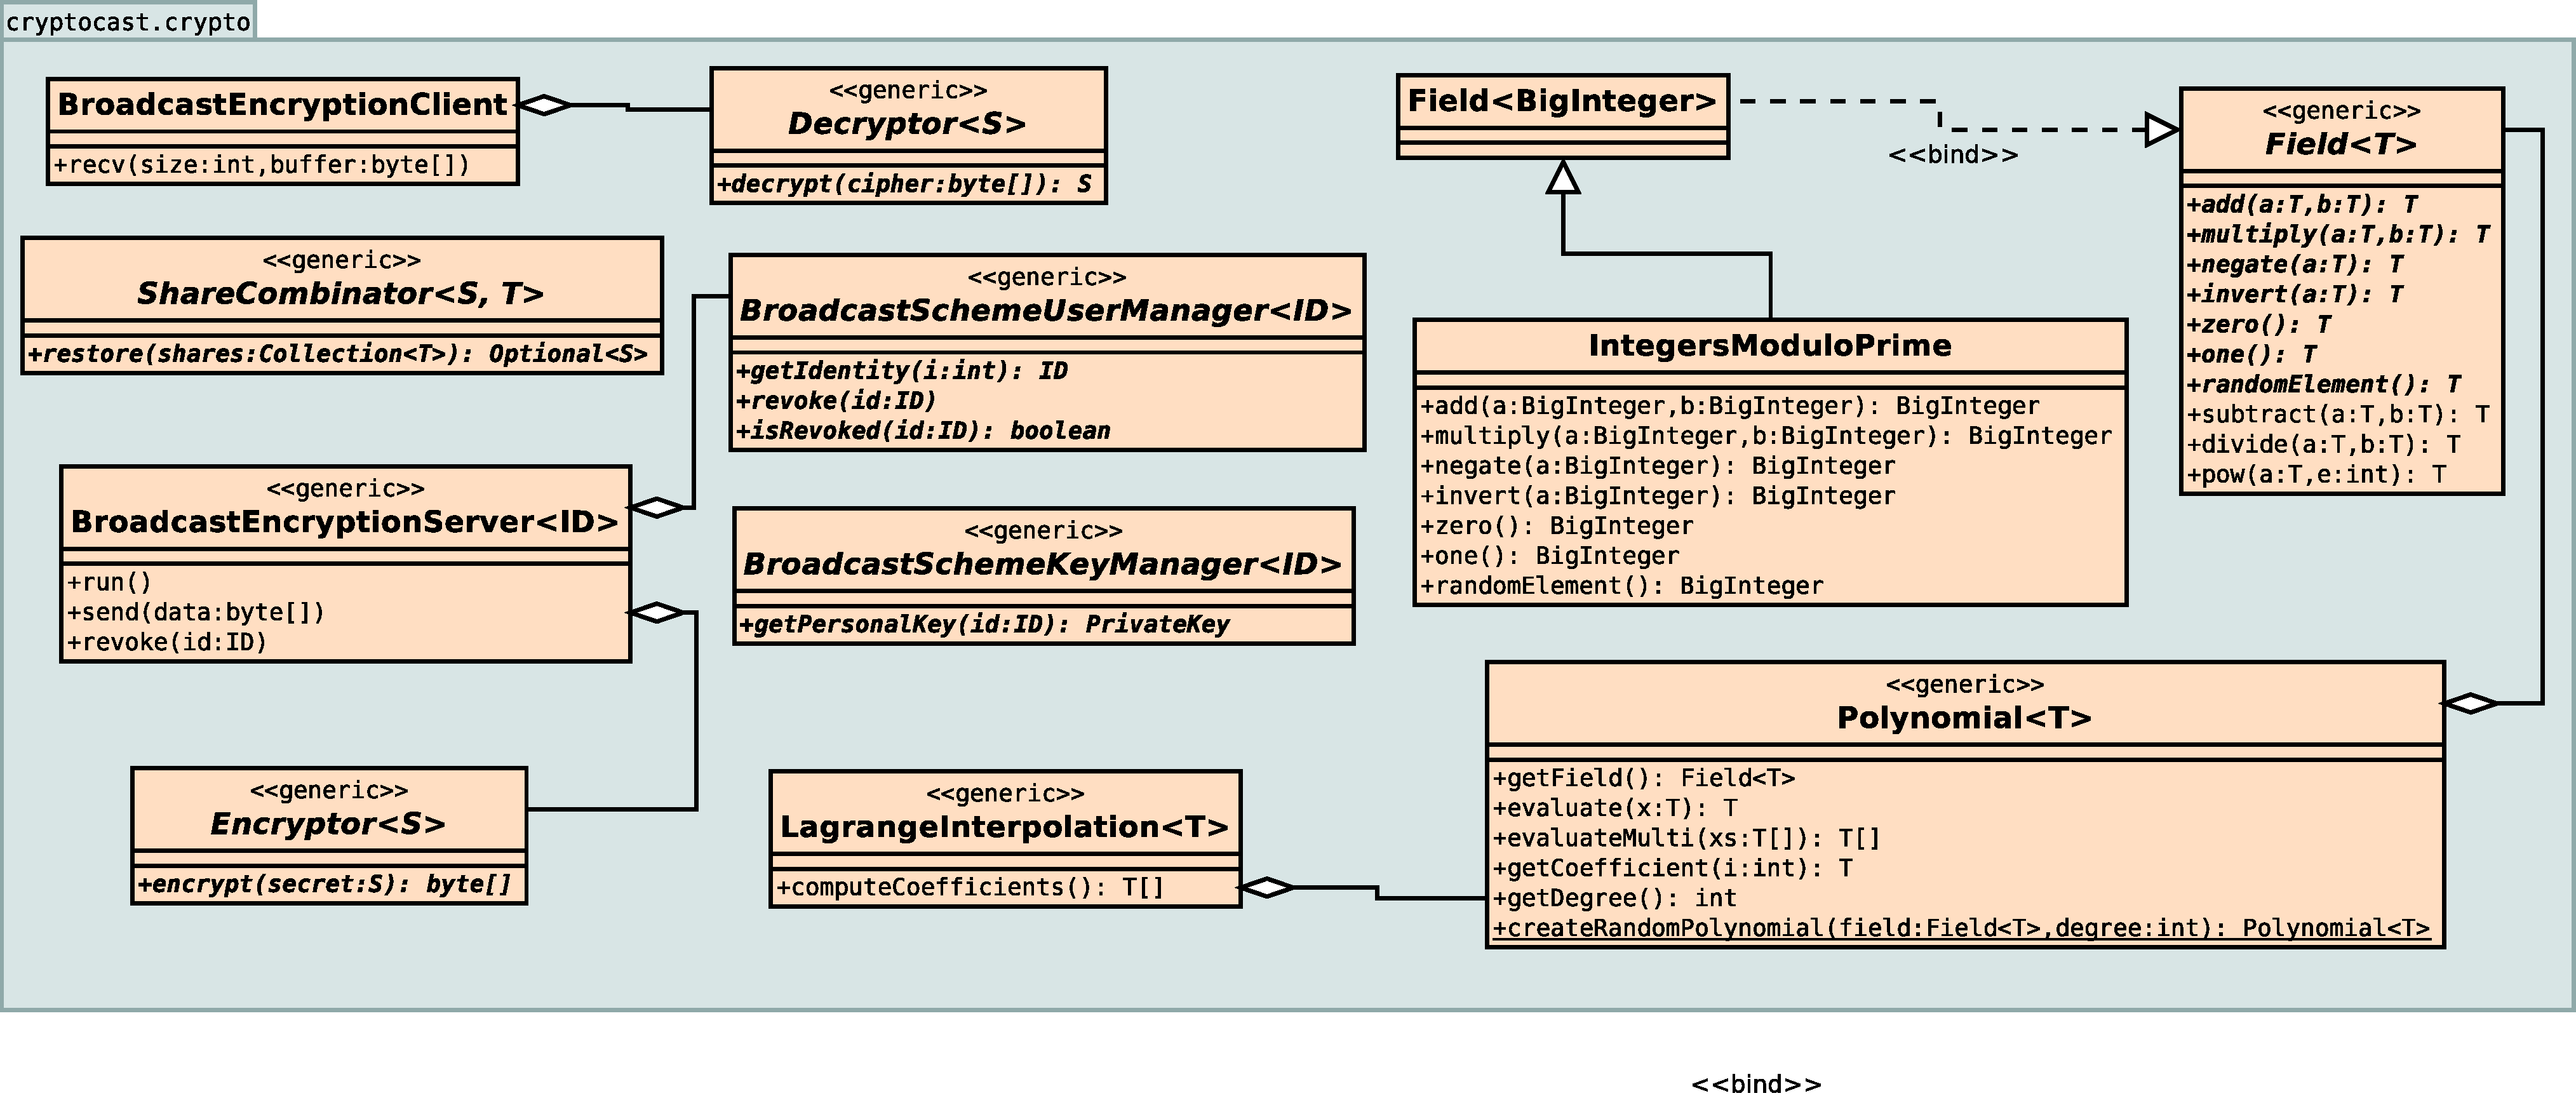
\includegraphics[width=450px]{class_diagrams/cryptocast_crypto.pdf}
\end{minipage}

\subsubsection{Class \lstinline|LagrangeInterpolation<T>|}
Performs a lagrange interpolation of a polynomial \\
\noindent\begin{minipage}[t]{5cm}
\vspace{0.3em}
\hspace*{2em}
\begin{tikzpicture}
\umlclass[]{LagrangeInterpolation<T>}{

}{
+ computeCoefficients() : T[]
}
\end{tikzpicture}
\vspace{0.3em}
\end{minipage}

\begin{itemize}
\item \lstinline|<T>|: The type of items of the polynomial's field
\end{itemize}



\textbf{\sffamily Constructors}
\begin{itemize}
\item \lstinline|public| \lstinline|LagrangeInterpolation|\lstinline|(Polynomial<T> poly)|\\ \\[-0.6em]
Initializes the algorithm
\begin{itemize}
\item \lstinline|poly|: The polynomial to interpolate
\end{itemize}



\end{itemize}


\textbf{\sffamily Methods}
\begin{itemize}
\item \lstinline|public T[]| \lstinline|computeCoefficients|\lstinline|()|\\ \\[-0.6em]
\emph{Returns:} The lagrange coefficients of the associated polynomial



\end{itemize}

\subsubsection{Class \lstinline|IntegersModuloPrime|}
The field $\mathbb{Z}/p\mathbb{Z}$ of integers modulo a prime $p$ \\
\noindent\begin{minipage}[t]{5cm}
\vspace{0.3em}
\hspace*{2em}
\begin{tikzpicture}
\umlclass[]{IntegersModuloPrime}{

}{
+ add(a : BigInteger, b : BigInteger) : BigInteger \\ + multiply(a : BigInteger, b : BigInteger) : BigInteger \\ + negate(a : BigInteger) : BigInteger \\ + invert(a : BigInteger) : BigInteger \\ + zero() : BigInteger \\ + one() : BigInteger \\ + randomElement() : BigInteger
}
\end{tikzpicture}
\vspace{0.3em}
\end{minipage}



\textbf{\sffamily Superclasses and Interfaces}
\begin{itemize}
\item \lstinline|cryptocast.crypto.Field<BigInteger>|
\end{itemize}


\textbf{\sffamily Constructors}
\begin{itemize}
\item \lstinline|public| \lstinline|IntegersModuloPrime|\lstinline|(BigInteger p)|\\ \\[-0.6em]
Initializes the field
\begin{itemize}
\item \lstinline|p|: A prime number
\end{itemize}



\end{itemize}


\textbf{\sffamily Methods}
\begin{itemize}
\item \lstinline|public BigInteger| \lstinline|add|\lstinline|(BigInteger a, BigInteger b)| \\[-0.6em]




\item \lstinline|public BigInteger| \lstinline|multiply|\lstinline|(BigInteger a, BigInteger b)| \\[-0.6em]




\item \lstinline|public BigInteger| \lstinline|negate|\lstinline|(BigInteger a)| \\[-0.6em]




\item \lstinline|public BigInteger| \lstinline|invert|\lstinline|(BigInteger a)| \\[-0.6em]




\item \lstinline|public BigInteger| \lstinline|zero|\lstinline|()| \\[-0.6em]




\item \lstinline|public BigInteger| \lstinline|one|\lstinline|()| \\[-0.6em]




\item \lstinline|public BigInteger| \lstinline|randomElement|\lstinline|()| \\[-0.6em]




\end{itemize}

\subsubsection{Class \lstinline|Polynomial<T>|}
A polynomial $P$ over a field \\
\noindent\begin{minipage}[t]{5cm}
\vspace{0.3em}
\hspace*{2em}
\begin{tikzpicture}
\umlclass[]{Polynomial<T>}{

}{
+ getField() : Field<T> \\ + evaluate(x : T) : T \\ + evaluateMulti(xs : T[]) : T[] \\ + getCoefficient(i : int) : T \\ + getDegree() : int \\ \umlstatic{+ createRandomPolynomial(field : Field<T>, degree : int) : Polynomial<T>}
}
\end{tikzpicture}
\vspace{0.3em}
\end{minipage}

\begin{itemize}
\item \lstinline|<T>|: The type of the field's elements
\end{itemize}



\textbf{\sffamily Constructors}
\begin{itemize}
\item \lstinline|public| \lstinline|Polynomial|\lstinline|(Field<T> field, T[] coefficients)|\\ \\[-0.6em]
Initializes a polynomial
\begin{itemize}
\item \lstinline|field|: An instance of the field over which the polynomial is formed
\item \lstinline|coefficients|: The coefficients $c_i$ of the polynomial ($0 \leq i \leq n$).
 The polynomial is defined as $P(x) := \sum_{i=0}^n c_i x^i = c_0 + c_1
 x + ... + c_n x^n$
\end{itemize}



\end{itemize}


\textbf{\sffamily Methods}
\begin{itemize}
\item \lstinline|public Field<T>| \lstinline|getField|\lstinline|()|\\ \\[-0.6em]
\emph{Returns:} The field associated with this polynomial



\item \lstinline|public T| \lstinline|evaluate|\lstinline|(T x)|\\ \\[-0.6em]
Evaluates the polynomial at a single point x.
\begin{itemize}
\item \lstinline|x|: The
\end{itemize}

\emph{Returns:} P(x)

\item \lstinline|public T[]| \lstinline|evaluateMulti|\lstinline|(T[] xs)|\\ \\[-0.6em]
Evaluates the polynomial at multiple points in time complexity $\Theta(n\cdot\log
 n)$ where $n$ is the degree of the polynomial
\begin{itemize}
\item \lstinline|xs|: The points $x_i$ to evaluate
\end{itemize}

\emph{Returns:} The array a defined by $a_i := P(x_i)$

\item \lstinline|public T| \lstinline|getCoefficient|\lstinline|(int i)|\\ \\[-0.6em]
\emph{Returns:} $c_i$
\begin{itemize}
\item \lstinline|i|: The index of the coefficient to get ($0 \leq i \leq n$), where
          $n$ is the degree of the polynomial
\end{itemize}



\item \lstinline|public int| \lstinline|getDegree|\lstinline|()|\\ \\[-0.6em]
\emph{Returns:} The degree of the polynomial



\item \lstinline|public static Polynomial<T>| \lstinline|createRandomPolynomial|\lstinline|(Field<T> field, int degree)|\\ \\[-0.6em]
Generates a random polynomial over the field
\begin{itemize}
\item \lstinline|field|: An instance of the field over which the polynomial is formed
\item \lstinline|degree|: The degree of the generated polynomial
\end{itemize}

\emph{Returns:} The generated polynomial

\end{itemize}

\subsubsection{Class \lstinline|Field<T>|}
Represents a field over values of type T \\
\noindent\begin{minipage}[t]{5cm}
\vspace{0.3em}
\hspace*{2em}
\begin{tikzpicture}
\umlclass[type=abstract]{Field<T>}{

}{
\umlvirt{+ add(a : T, b : T) : T} \\ \umlvirt{+ multiply(a : T, b : T) : T} \\ \umlvirt{+ negate(a : T) : T} \\ \umlvirt{+ invert(a : T) : T} \\ \umlvirt{+ zero() : T} \\ \umlvirt{+ one() : T} \\ \umlvirt{+ randomElement() : T} \\ + subtract(a : T, b : T) : T \\ + divide(a : T, b : T) : T \\ + pow(a : T, e : int) : T
}
\end{tikzpicture}
\vspace{0.3em}
\end{minipage}

\begin{itemize}
\item \lstinline|<T>|: The values we work on
\end{itemize}




\textbf{\sffamily Methods}
\begin{itemize}
\item \lstinline|public abstract T| \lstinline|add|\lstinline|(T a, T b)|\\ \\[-0.6em]
Adds two elements of the field
\begin{itemize}
\item \lstinline|a|: first element
\item \lstinline|b|: second element
\end{itemize}

\emph{Returns:} The value $a + b$

\item \lstinline|public abstract T| \lstinline|multiply|\lstinline|(T a, T b)|\\ \\[-0.6em]
Multiplies two elements of the field
\begin{itemize}
\item \lstinline|a|: first element
\item \lstinline|b|: second element
\end{itemize}

\emph{Returns:} The value $a \cdot b$

\item \lstinline|public abstract T| \lstinline|negate|\lstinline|(T a)|\\ \\[-0.6em]
\emph{Returns:} The additive inverse $-a$ of $a$
\begin{itemize}
\item \lstinline|a|: An element of the field
\end{itemize}



\item \lstinline|public abstract T| \lstinline|invert|\lstinline|(T a)|\\ \\[-0.6em]
\emph{Returns:} The multiplicative inverse $a^{-1}$ of $a$
\begin{itemize}
\item \lstinline|a|: An element of the field
\end{itemize}



\item \lstinline|public abstract T| \lstinline|zero|\lstinline|()|\\ \\[-0.6em]
\emph{Returns:} The zero element of the field



\item \lstinline|public abstract T| \lstinline|one|\lstinline|()|\\ \\[-0.6em]
\emph{Returns:} The one element of the field



\item \lstinline|public abstract T| \lstinline|randomElement|\lstinline|()|\\ \\[-0.6em]
\emph{Returns:} A random element of the field



\item \lstinline|public T| \lstinline|subtract|\lstinline|(T a, T b)|\\ \\[-0.6em]
Subtracts two elements of the field
\begin{itemize}
\item \lstinline|a|: first element
\item \lstinline|b|: second element
\end{itemize}

\emph{Returns:} The value $a - b$

\item \lstinline|public T| \lstinline|divide|\lstinline|(T a, T b)|\\ \\[-0.6em]
Divides two elements of the field
\begin{itemize}
\item \lstinline|a|: first element
\item \lstinline|b|: second element
\end{itemize}

\emph{Returns:} The value $\frac{a}{b}$

\item \lstinline|public T| \lstinline|pow|\lstinline|(T a, int e)|\\ \\[-0.6em]
Raises an element of the field to an integer power
\begin{itemize}
\item \lstinline|a|: The element of the field
\item \lstinline|e|: The exponent
\end{itemize}

\emph{Returns:} The value $a^e$

\end{itemize}

\subsubsection{Class \lstinline|BroadcastEncryptionServer<ID>|}
The server side of a broadcast encryption scheme. \\
\noindent\begin{minipage}[t]{5cm}
\vspace{0.3em}
\hspace*{2em}
\begin{tikzpicture}
\umlclass[]{BroadcastEncryptionServer<ID>}{

}{
+ run() \\ + send(data : byte[]) \\ + revoke(id : ID)
}
\end{tikzpicture}
\vspace{0.3em}
\end{minipage}

\begin{itemize}
\item \lstinline|<ID>|: The type of the identities
\end{itemize}


\textbf{\sffamily Superclasses and Interfaces}
\begin{itemize}
\item \lstinline|cryptocast.comm.OutChannel|
\item \lstinline|java.lang.Runnable|
\end{itemize}


\textbf{\sffamily Constructors}
\begin{itemize}
\item \lstinline|public| \lstinline|BroadcastEncryptionServer|\lstinline|(MessageOutChannel inner, BroadcastSchemeUserManager<ID> context, Encryptor<BigInteger> enc)|\\ \\[-0.6em]
Initializes a broadcast encryption server.
\begin{itemize}
\item \lstinline|inner|: The message-based communication channel to send outgoing data to
\item \lstinline|context|: The user management context
\item \lstinline|enc|: The encryption context
\end{itemize}



\end{itemize}


\textbf{\sffamily Methods}
\begin{itemize}
\item \lstinline|public void| \lstinline|run|\lstinline|()|\\ \\[-0.6em]
Run the worker that handles periodic group key broadcasts and sends
 queued data packages.



\item \lstinline|public void| \lstinline|send|\lstinline|(byte[] data)|\\ \\[-0.6em]
Send plaintext data to the channel. It will be encryted and broadcasted
 on the fly.
\begin{itemize}
\item \lstinline|data|: The data to send
\end{itemize}



\item \lstinline|public void| \lstinline|revoke|\lstinline|(ID id)|\\ \\[-0.6em]
Revoke a user.
\begin{itemize}
\item \lstinline|id|: The identity of the user
\end{itemize}



\end{itemize}

\subsubsection{Class \lstinline|BroadcastEncryptionClient|}
The client side of a broadcast encryption scheme. \\
\noindent\begin{minipage}[t]{5cm}
\vspace{0.3em}
\hspace*{2em}
\begin{tikzpicture}
\umlclass[]{BroadcastEncryptionClient}{

}{
+ recv(size : int, buffer : byte[])
}
\end{tikzpicture}
\vspace{0.3em}
\end{minipage}



\textbf{\sffamily Superclasses and Interfaces}
\begin{itemize}
\item \lstinline|cryptocast.comm.InChannel|
\end{itemize}


\textbf{\sffamily Constructors}
\begin{itemize}
\item \lstinline|public| \lstinline|BroadcastEncryptionClient|\lstinline|(MessageInChannel inner, Decryptor<BigInteger> dec)|\\ \\[-0.6em]
Initializes a broadcast encryption client.
\begin{itemize}
\item \lstinline|inner|: The message-based underlying communication channel.
\item \lstinline|dec|: The decryption context
\end{itemize}



\end{itemize}


\textbf{\sffamily Methods}
\begin{itemize}
\item \lstinline|public void| \lstinline|recv|\lstinline|(int size, byte[] buffer)|\\ \\[-0.6em]
Receive data from the channel. It is decrypted on the fly.
\begin{itemize}
\item \lstinline|size|: amount of bytes to receive
\item \lstinline|buffer|: the target buffer
\end{itemize}



\end{itemize}

\subsubsection{Interface \lstinline|Decryptor<S>|}
A strategy to decrypt a single secret \\
\noindent\begin{minipage}[t]{5cm}
\vspace{0.3em}
\hspace*{2em}
\begin{tikzpicture}
\umlclass[type=abstract]{Decryptor<S>}{

}{
\umlvirt{+ decrypt(cipher : byte[]) : S}
}
\end{tikzpicture}
\vspace{0.3em}
\end{minipage}

\begin{itemize}
\item \lstinline|<S>|: the type of the secret
\end{itemize}




\textbf{\sffamily Methods}
\begin{itemize}
\item \lstinline|public S| \lstinline|decrypt|\lstinline|(byte[] cipher)|\\ \\[-0.6em]
Decrypts a secret.
\begin{itemize}
\item \lstinline|cipher|: The encrypted secret
\end{itemize}

\emph{Returns:} The decrypted secret

\end{itemize}

\subsubsection{Interface \lstinline|BroadcastSchemeUserManager<ID>|}
Manages a set of user identites \\
\noindent\begin{minipage}[t]{5cm}
\vspace{0.3em}
\hspace*{2em}
\begin{tikzpicture}
\umlclass[type=abstract]{BroadcastSchemeUserManager<ID>}{

}{
\umlvirt{+ getIdentity(i : int) : ID} \\ \umlvirt{+ revoke(id : ID)} \\ \umlvirt{+ isRevoked(id : ID) : boolean}
}
\end{tikzpicture}
\vspace{0.3em}
\end{minipage}

\begin{itemize}
\item \lstinline|<ID>|: The type of the identities
\end{itemize}




\textbf{\sffamily Methods}
\begin{itemize}
\item \lstinline|public ID| \lstinline|getIdentity|\lstinline|(int i)|\\ \\[-0.6em]
\emph{Returns:} The identity with the given index
\begin{itemize}
\item \lstinline|i|: An index
\end{itemize}



\item \lstinline|public void| \lstinline|revoke|\lstinline|(ID id)|\\ \\[-0.6em]
Revokes a user
\begin{itemize}
\item \lstinline|id|: The identity of the user
\end{itemize}



\item \lstinline|public boolean| \lstinline|isRevoked|\lstinline|(ID id)|\\ \\[-0.6em]
\emph{Returns:} whether the user is revoked
\begin{itemize}
\item \lstinline|id|: The identity of the user
\end{itemize}



\end{itemize}

\subsubsection{Interface \lstinline|Encryptor<S>|}
A strategy to encrypt a single secret \\
\noindent\begin{minipage}[t]{5cm}
\vspace{0.3em}
\hspace*{2em}
\begin{tikzpicture}
\umlclass[type=abstract]{Encryptor<S>}{

}{
\umlvirt{+ encrypt(secret : S) : byte[]}
}
\end{tikzpicture}
\vspace{0.3em}
\end{minipage}

\begin{itemize}
\item \lstinline|<S>|: the type of the secret
\end{itemize}




\textbf{\sffamily Methods}
\begin{itemize}
\item \lstinline|public byte[]| \lstinline|encrypt|\lstinline|(S secret)|\\ \\[-0.6em]
Encrypts a secret
\begin{itemize}
\item \lstinline|secret|: the secret
\end{itemize}

\emph{Returns:} The cipher text

\end{itemize}

\subsubsection{Interface \lstinline|BroadcastSchemeKeyManager<ID>|}
Manages the private keys of a set of users. \\
\noindent\begin{minipage}[t]{5cm}
\vspace{0.3em}
\hspace*{2em}
\begin{tikzpicture}
\umlclass[type=abstract]{BroadcastSchemeKeyManager<ID>}{

}{
\umlvirt{+ getPersonalKey(id : ID) : PrivateKey}
}
\end{tikzpicture}
\vspace{0.3em}
\end{minipage}

\begin{itemize}
\item \lstinline|<ID>|: The type of the user identities
\end{itemize}




\textbf{\sffamily Methods}
\begin{itemize}
\item \lstinline|public PrivateKey| \lstinline|getPersonalKey|\lstinline|(ID id)|\\ \\[-0.6em]
\emph{Returns:} The private key of the user
\begin{itemize}
\item \lstinline|id|: The identity to look up
\end{itemize}



\end{itemize}

\subsubsection{Interface \lstinline|ShareCombinator<S, T>|}
Implements a strategy to restore a secret from a number of shares. \\
\noindent\begin{minipage}[t]{5cm}
\vspace{0.3em}
\hspace*{2em}
\begin{tikzpicture}
\umlclass[type=abstract]{ShareCombinator<S, T>}{

}{
\umlvirt{+ restore(shares : Collection<T>) : Optional<S>}
}
\end{tikzpicture}
\vspace{0.3em}
\end{minipage}

\begin{itemize}
\item \lstinline|<S>|: The type of the secret
\item \lstinline|<T>|: The type of the shares
\end{itemize}




\textbf{\sffamily Methods}
\begin{itemize}
\item \lstinline|public Optional<S>| \lstinline|restore|\lstinline|(Collection<T> shares)|\\ \\[-0.6em]
Restores a secret from several shares.

\emph{Returns:} The reconstructed secret or absent if the information represented
 by the given shares is insufficient to restore it.

\end{itemize}


